\documentclass[a4paper, 12pt]{scrartcl}

\usepackage[T1]{fontenc}
\usepackage{lmodern}
\usepackage[french]{babel}
\usepackage{amsmath}
\usepackage{siunitx}
\usepackage{graphicx}
\graphicspath{{./images/}}
\usepackage{hyperref}
\hypersetup{
    colorlinks = true,
    urlcolor = blue!60!black,
    linkcolor = black
}
\usepackage{tikz}
\usetikzlibrary{shapes.misc, calc}
%\usepackage{showframe}

\begin{document}
\title{Sujet de Grand Oral - Simulation de l'atterissage de Apollo 11 sur la Lune }
\author{Elliot Jullier}
\date{\today}
\maketitle

\pagenumbering{roman}
\tableofcontents

\newpage
\pagenumbering{arabic}




\subsection{- Introduction}
Après les multiples victoires technologiques de l'URSS dans la course des étoiles, premièrement le satellite de Spoutnik 1 en 1957 choque le monde ainsi que Laika, ensuite avec Yuri Gagarin, premier homme dans l'espace ; 
les victoires consécutives tel que la premiere sortie extravéhiculaire. 
\\
\\
\indent
Le Président Kennedy annonca la participation des Etats-Unis de cette compétition spatiale en 
Septembre 1962 qui promet de mettre un homme sur la Lune avant la fin de la décennie. 
Le 16 Juillet 1969, Apollo 11, contenant les astronautes Neil Armstrong, Edwin ``Buzz'' Aldrin et Michael Collins
part de la Terre, l'orbite plusieurs fois et puis envoie une petite navette contenant ces trois astronautes vers la Lune.
En arrivant dans la sphère d'influence (région de l'espace ou un certain corps céleste est la force dominante) de la Lune trois jours plus tard, la vitesse est bien trop grande et le vaisseau n'orbite pas la Lune, il faut effectuer un premier ajustement 
pour permettre aux astronautes de se situer à une orbite de $111$ km au dessus de la surface lunaire.
\\
\\
\indent
On a construit une simulation qui cherche à mieux comprendre comment l'atterissage sur la Lune
s'est produite, cette mission a été choisie grâce à sa signification historique et les
données importantes récoltées. 


% Add references when values are calculated to the appropriate formula in part 2
\section{- Etapes de l'Atterissage}
\subsection{- Parametres initiaux : Orbite Circulaire}
Nous cherchons à modeliser la mission de Apollo 11 du 20-21 Juillet 1969 comme exemple d'atterissage
de fusée sur la Lune car cela donne un modèle avec beaucoups de statistiques grace à sa sigificance 
historique. 
\\
\\
\indent
Il y a deux capsules en orbite a $111$ km d'altitude au-dessus de la surface de la Lune: la \emph{Command and Service Module} - CSM,
partie qui reste en orbite avec l'astronaut Michael Collins, et le \emph{Lunar Module} - LM, avec Neil Armstrong et Edwin `Buzz' Aldrin.
En sachant que les deux parties attachés sont en orbite circulaire a une altitude de $111$ km on peut calculer
la vitesse initiale $\| \overrightarrow{v} \| = 1628,9\ \si{m.s^{-1}}$. 

\begin{center}
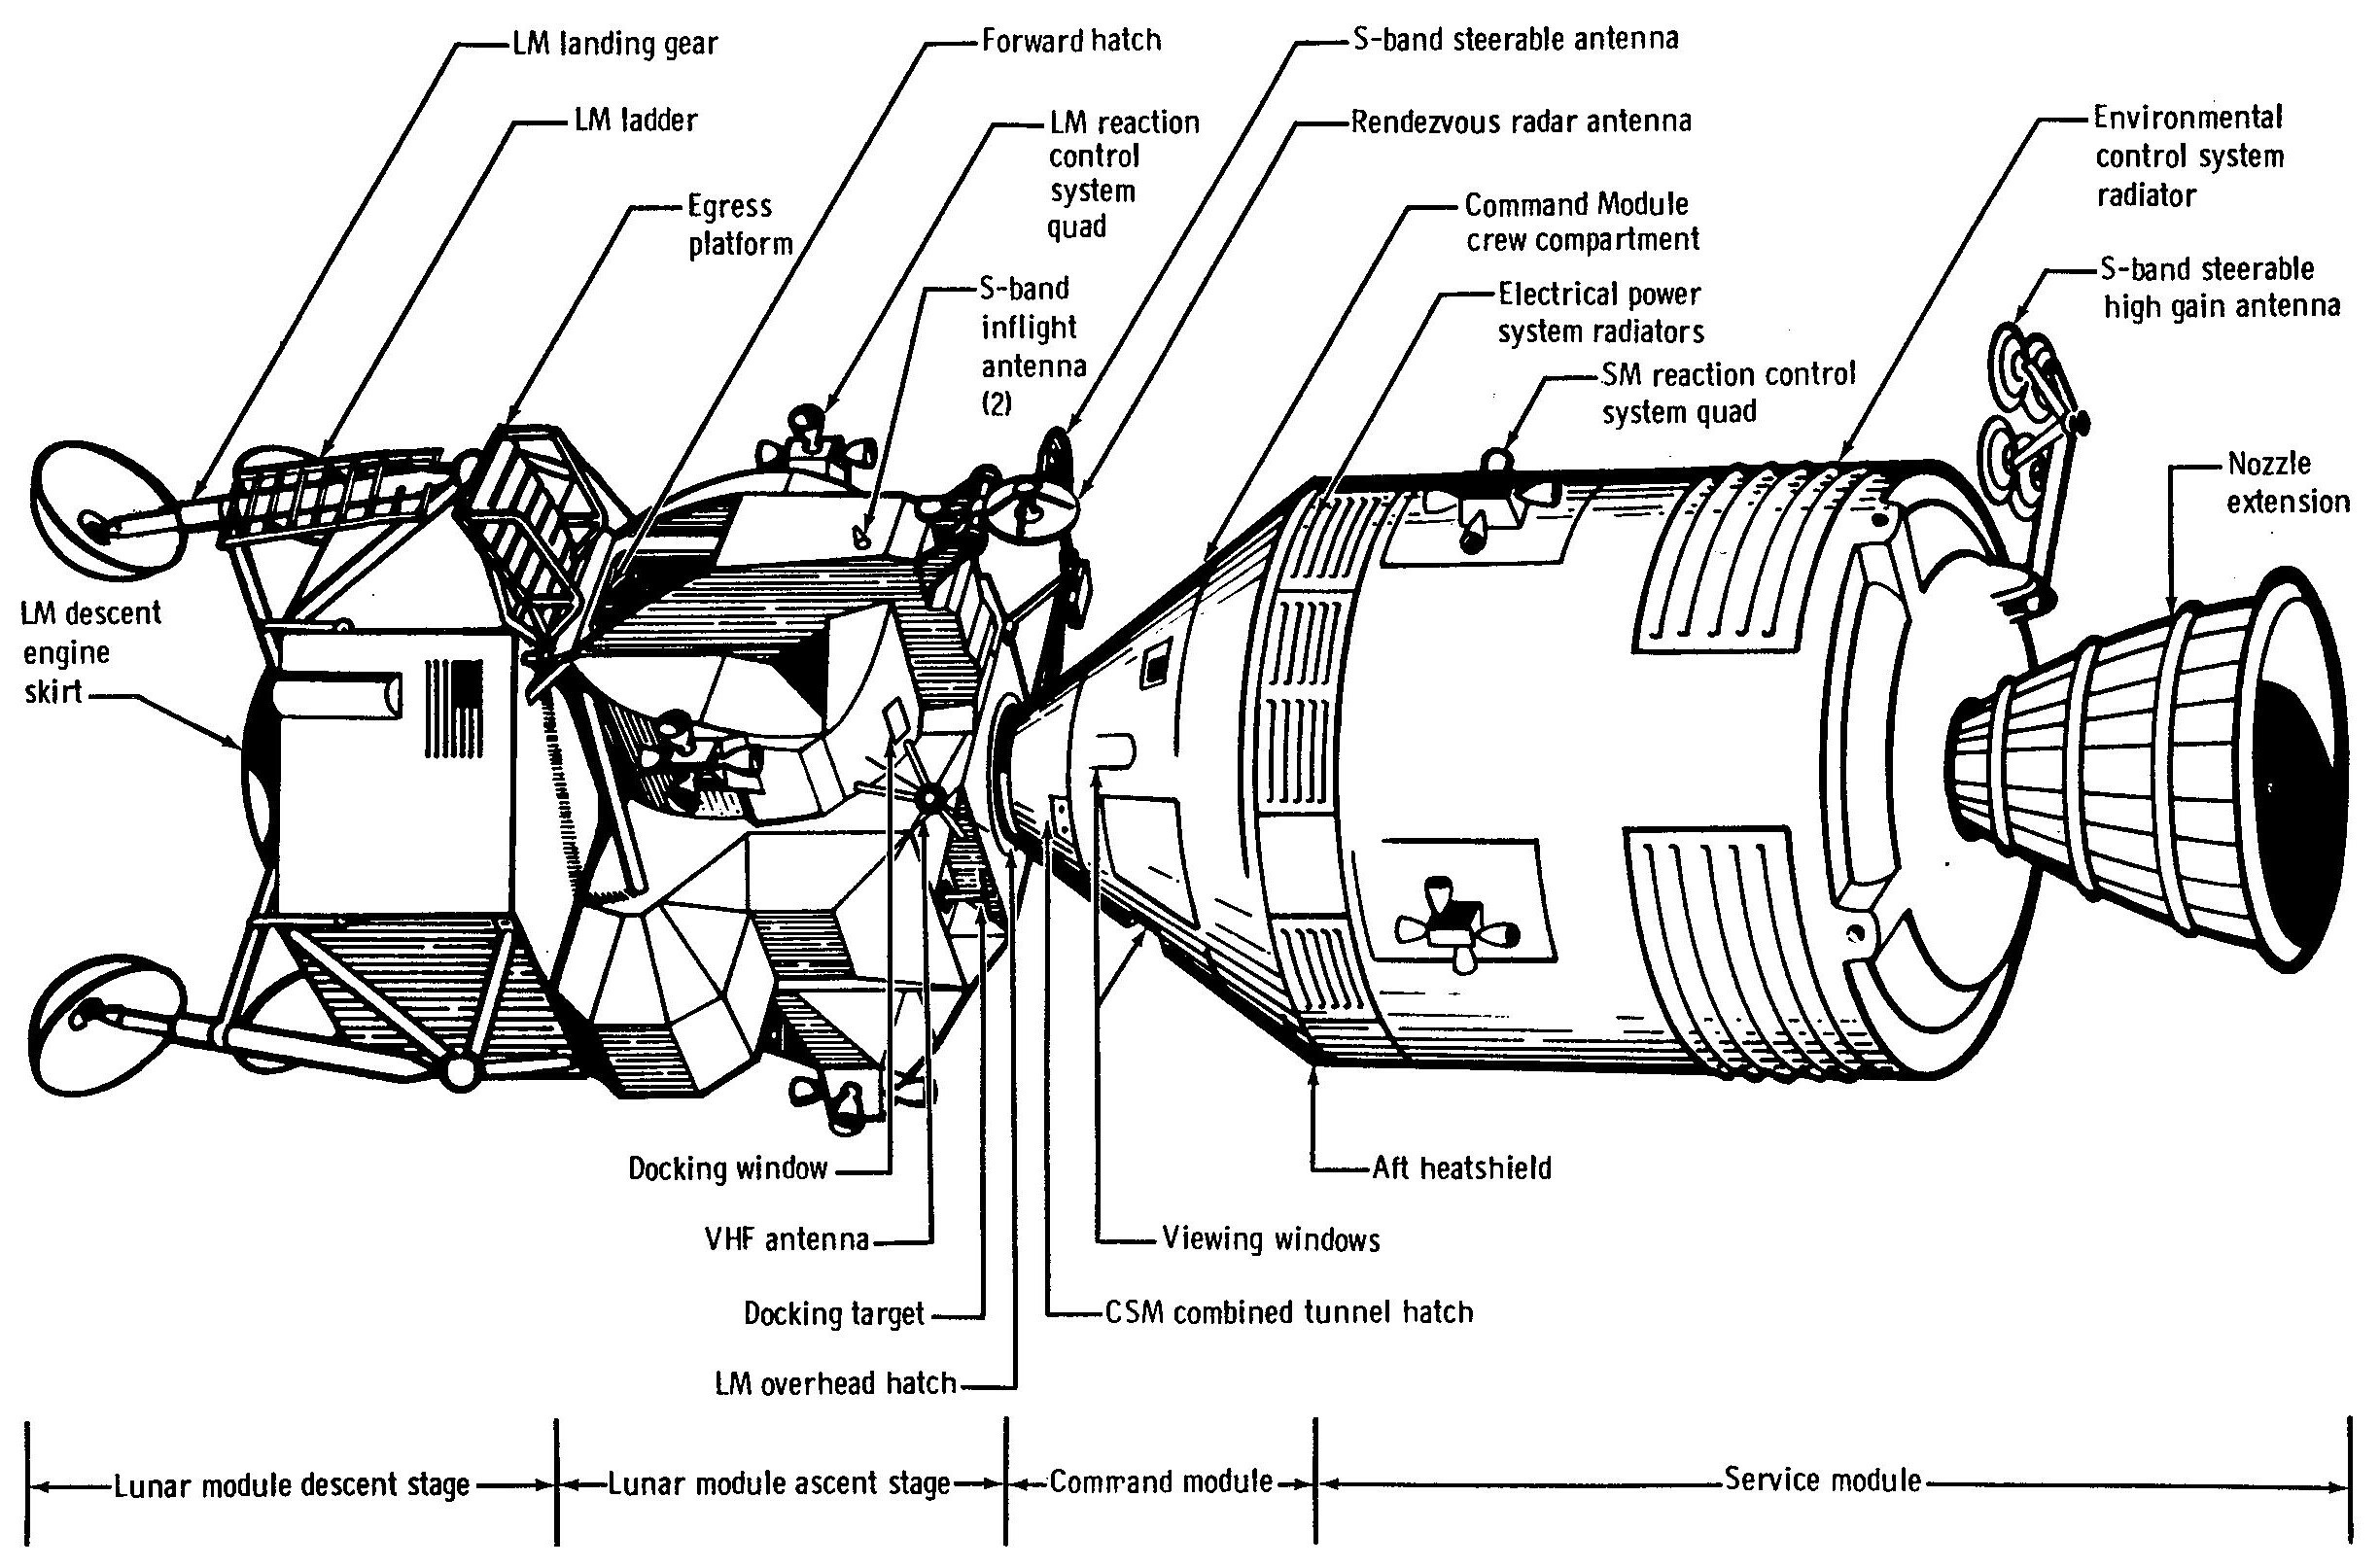
\includegraphics[width=300pt]{CSM+LM_Schema}
\\
\vspace{5mm}
\emph{Figure 1 - Schéma du CSM et LM}
\end{center}

\subsection{- Transfer de Hohmann : Ellipse Intermédiaire}
On sépare ensuite les deux modules et on assure une distance d'au moins $10$ m entre eux, puis on pointe
le moteur de la LM dans la direction du vecteur vitesse mais dans le sens opposé. On effectue un changement $\Delta \overrightarrow{v} = -21,81\ \si{m.s^{-1}}$, 
qui met la fusée en une orbite elliptique avec un aposélene (point où l'altitude est maximale) à la location du changement (à $111$ km) et
avec un perisélene (point où l'altitude est minimale) à 180° de rotation autour du corps céleste et une altitude de $15,2$ km. 
\\
\begin{center}
\begin{tikzpicture}
    \def \largeRadius {3}
    \def \smallRadius {1}
    % Fake Moon
    \fill[black!30] (0,0) circle (0.2 * \largeRadius); 
    % Center point
    \draw [ultra thick] (-0.05*\largeRadius,-0.05*\largeRadius) -- (0.05*\largeRadius,0.05*\largeRadius);  
    \draw [ultra thick] (-0.05*\largeRadius, 0.05*\largeRadius) -- (0.05*\largeRadius,-0.05*\largeRadius);
    \node at (0.12*\largeRadius,-0.06*\largeRadius) {O}; 
    % Primary Orbit
    \draw[thick] (0,0) circle (\largeRadius); 
    % Intermediary Ellipse
    \draw[thick] ({(\largeRadius - \smallRadius)*0.5},0) + (0:{(\largeRadius + \smallRadius)*0.5} and 1.5) arc (0:180:{(\largeRadius + \smallRadius)*0.5} and 1.5);  % Filled in semi-circle
    \draw[dashed] ({(\largeRadius - \smallRadius)*0.5},0) + (180:{(\largeRadius + \smallRadius)*0.5} and 1.5) arc (180:360:{(\largeRadius + \smallRadius)*0.5} and 1.5); % Dashed semi-circle
    % Theoretical Small Orbit
    \draw[dotted] (0,0) circle (\smallRadius); 
    % Aposelene Point
    \draw [thick] (0.95*\largeRadius, -0.05 * \largeRadius) -- (1.05 * \largeRadius, 0.05 * \largeRadius);
    \draw [thick] (0.95 * \largeRadius, 0.05 * \largeRadius) -- (1.05 * \largeRadius, -0.05 * \largeRadius);
    \node at (1.15 * \largeRadius, 0) {\small A \normalsize};
    % Periselene Point
    \draw [thick] (-\smallRadius - 0.05* \largeRadius, -0.05 * \largeRadius) -- (-\smallRadius + 0.05 * \largeRadius, 0.05 * \largeRadius);
    \draw [thick] (-\smallRadius - 0.05 * \largeRadius, 0.05 * \largeRadius) -- (-\smallRadius + 0.05 * \largeRadius, -0.05 * \largeRadius);
    \node at (-0.48 * \largeRadius, 0) {\small P \normalsize};
    % Indication arrows
    \draw [ultra thick,->] (0, \largeRadius) -- (-0.7* \largeRadius, \largeRadius) node[midway, above, align=center, xshift = -0.2cm] {$\overrightarrow{v_{c1}}$};
    \draw [ultra thick, ->] (\largeRadius, 0) -- (\largeRadius, 0.7 * \largeRadius) node[midway, right, align=center] {$\overrightarrow{v_{\text{A}}}$};
    \draw [ultra thick, ->] (\largeRadius, 0) -- (\largeRadius, -0.4 * \largeRadius) node[midway, right, align=center] {$\overrightarrow{\Delta v}$};
    \draw [ultra thick, ->] (-\smallRadius, 0) -- (-\smallRadius, -0.4 * \largeRadius) node[midway, left, align=center] {$\overrightarrow{v_{\text{P}}}$};
    % Legende
    \node[text width = 8cm] at (3 * \largeRadius, 0.75 * \largeRadius) {$A$ - L'aposélene pour l'orbite elliptique};
    \node[text width = 8cm] at (3 * \largeRadius, 0.45 * \largeRadius) {$P$ - Le périsélene pour l'orbite elliptique};
    \node[text width = 8cm] at (3 * \largeRadius, 0.15 * \largeRadius) {$\overrightarrow{v_{c1}}$ - La vitesse pour une orbite circulaire};
    \node[text width = 8cm] at (3 * \largeRadius, - 0.15 * \largeRadius) {$\overrightarrow{v_{\text{A}}}$ - La vitesse à A pour l'orbite elliptique};
    \node[text width = 8cm] at (3 * \largeRadius, - 0.45 * \largeRadius) {$\overrightarrow{v_{\text{P}}}$ - La vitesse à P pour l'orbite elliptique};
    \node[text width = 8cm] at (3 * \largeRadius, - 0.75 * \largeRadius) {$\overrightarrow{\Delta v}$ - Le $\Delta v$ nécesaire pour passer de l'orbite circulaire à l'orbite elliptique};
    \draw (3 * \largeRadius - 4.5, -0.75 * \largeRadius - 0.75) -- (3 * \largeRadius -4.5, 0.75 * \largeRadius + 0.5) -- (3 * \largeRadius +4.5, 0.75 * \largeRadius + 0.5) -- (3 * \largeRadius + 4.5, -0.75 * \largeRadius -0.75) -- (3 * \largeRadius -4.5, -0.75 * \largeRadius - 0.75);


\end{tikzpicture}
\\
\vspace{5mm}
\emph{Figure 2 - Transfer de Hohmann (partiel) pour approcher la Lune}
\end{center}
\vspace{5mm}

Normalement, en arrivant au périsélene, on effectue une rotation pour pouvoir ralentir de nouveau le vaisseau
et circulariser l'orbite (pour que l'eccentricité soit de 0 et de garder l'altitude du périsélene).

\subsection{- Phases de Descente}
La phase de déscente est plus dur à modeliser car elle varie dépendant des circonstances, peut changer a tout moment,
et surtout n'a pas de bonnes equations pour modeliser la vitesse mais plutôt des lignes directrices à suivre - 
il ne faut pas oublier que seuls les meilleurs pilotes pouvaient devenir astronautes et donc leur capacité surpasser de loins
les ordinateurs de l'époque.

\subsubsection{- Phase de Freinage}
On commence a une altitude de $15,2$ km avec une vitesse de $\overrightarrow{v_{\text{P}}} = 1694,6\ \si{m.s^{-1}}$ qui est entierement horizontale (seulement au périsélene) et qui a une vitesse 
verticale négligeable. On se situe environ $480$ km (à vol d'oiseau) du site d'atterisage.
\\ \\ \indent
Cette phase a comme but de ralentir majoritairement la vitesse horizontale, 
mais en ralentissant, la gravité commence à avoir plus d'emprise 
et la vitesse est trop basse pour pouvoir `dépasser' la Lune (cf. \href{https://fr.wikipedia.org/wiki/Canon_de_Newton}{Le Canon de Newton})

\subsubsection{- Phase de Repérage}
Une fois qu'on atteint environ $2,95$ km d'altitude (on situe maintenant à $10$ km du site d'atterissage à vol d'oiseau), il faut être au alentours de $150\ \si{m.s^{-1}}$
horizontalement, et $45\ \si{m.s^{-1}}$ verticale, ce qui donne une vitesse totale de $156,6\ \si{m.s^{-1}}$.
\\ \\ \indent
Cette phase a comme but de finir de ralentir la vitesse horizontale, mais aussi d'eviter une trop
forte accéleration vers le corps céleste. Elle sert aussi de trouver le lieu d'atterissage, notamment pendant
la mission d'Apollo 11, Neil Armstrong a du survoler le lieu d'atterissage prévu à cause d'un
champ de rochers.

\subsubsection{- Phase d'atterissage}
En arrivant a $150$ m d'altitude et  jusqu'à $600$ m de distance horizontale du  
site d'atterisage, il faut $20-0\ \si{m.s^-1}$ de vitesse horizontale et $8-1\ \si{m.s^{-1}}$ verticalement.
\\
Comme règle générale, il faut que la vitesse verticale soit un dixième de l'altitude, sauf les derniers mètres ou il faut
s'assurer un atterisage qui n'endommage des parties importantes tel que le moteur de remonté, les expériences et evidemment les
astronautes. 



\newpage
\section{- La méchanique dans le modèle}
\subsection{- Implementation de la position, vitesse et acceleration}
\subsubsection{- Relations physique}
Dans le chapitre de la méchanique, on a vu la relation entre les vecteurs
de position, vitesse et acceleration:
\\

%\[\overrightarrow{OM} \begin{pmatrix} x \\ y \\ z \end{pmatrix}\]
%\[\overrightarrow{v} \begin{pmatrix} x' \\ y' \\ z' \end{pmatrix} = \frac{d \overrightarrow{OM}}{d t} \begin{pmatrix} x \\ y \\ z \end{pmatrix} \]
\[\overrightarrow{a} \begin{pmatrix} x'' \\ y'' \\ z'' \end{pmatrix}
= \frac{d\overrightarrow{v}}{d t} \begin{pmatrix} x' \\ y' \\ z' \end{pmatrix}
= \frac{d^2 \overrightarrow{OM}}{d t^2}\begin{pmatrix} x \\ y \\ z \end{pmatrix}\]
\\
\\
\subsubsection{- Implementation par approximation}
La manière dont on a implémenté cette relation dans le programme est d'approximer la 
continuité et l'evolution des vecteurs en les approximants en valeurs discretes. 
\\ \\ \indent
Pour Unity le programme qu'on a utilisé pour la simulation, la valeur de temps entre chaque 'update' est de $\frac{1}{50}$ de seconde. 
\\ \\ \indent
On calcule l'acceleration et on `ajoute' ce vecteur a celui de la vitesse. Cela est comme faire: $v_{\text{future}} = v_{\text{courante}} + \Delta v$, cette action est répété
toute les $50^{\text{ième}}$ de seconde. On peut donc assimiler ajouter l'acceleration au vecteur vitesse comme ajoutant le $\Delta v$, 
les unités de l'acceleration en $\si{m.s^{-2}}$ multiplié par des $\si{s}$ donne des $\si{m.s^{-1}}$. En ajoutant le vecteur acceleration toute les $50^{\text{ième}}$ de seconde, 
on calcule le nouveau vecteur vitesse. 
\\ \\ \indent 
Similairement, pour la position, on prends la vitesse et on calcul la nouvelle position apres que la fusée
ait bougée pendant $\frac{1}{50}\ \si{s}$.

\subsection{- Evolution de l'acceleration}
Le moteur d'une fusée à un pourcentage de la 'puissance' maximale fourni une force
constante. 
\\
De plus:
\[F = ma \]
\indent
Par ailleur, le moteur d'une fusée brule la masse d'essence proportionellement a la `puissance' fournie.
Cela a pour consequence que la fusée a une augmentation d'acceleration au fur et 
à mesure qu'elle utilise son carburant. 

\subsection{- Force Appliqués sur la Fusée}
\subsubsection{- Orbite Circulaire}
Dans une orbite circulaire uniforme, il y a seul la force de gravité qui agit sur la fusée.
On a:
\[ \overrightarrow{F} = \frac{GMm}{r^2}\overrightarrow{n} \Leftrightarrow \overrightarrow{a} = \frac{GM}{r^2}\overrightarrow{n}\]
Avec $G\text{ : la constante gravitationelle en } \si{m^{3}.kg^{-1}.s^{-2}}\text{, } M \text{ : la masse de la Lune en } \si{kg} \text{, } 
\\ m \text{ : la masse de la fusée, } r \text{ : le rayon de l'orbite (} 
R_{\text{Lune}}\ +\ d_{\text{hauteur}} \text{ en } \si{m}  \text{), } \overrightarrow{n} \text{ : le vecteur unitaire} \\ \text{qui pointe vers le centre d'inertie de la Lune.}$
\\ \\ 
De plus on est dans un mouvement circulaire donc: $\overrightarrow{a} = \frac{v^2}{r}\overrightarrow{n}$
\\
Ce qui donne:
\[\frac{v^2}{r}\overrightarrow{n} = \overrightarrow{a} = \frac{GM}{r^2}\overrightarrow{n} \Leftrightarrow 
v^2 = \frac{GM}{r} \Leftrightarrow v = \sqrt{\frac{GM}{r}}\]
Avec la direction de la vitesse étant tangantielle à la trajectoire circulaire à prendre.
\\
\\
\begin{center}
    \begin{tikzpicture}
        \def \radius {2}; %cm
        \def \arrowLength {1.5}; %cm
        \def \innerArrowLength {1};
        \draw (0,0) circle (\radius);
        \fill[black!30] (0,0) circle (0.12*\radius);
        \draw [ultra thick] (-0.06*\radius,-0.06*\radius) -- (0.06*\radius,0.06*\radius);
        \draw [ultra thick] (-0.06*\radius, 0.06*\radius) -- (0.06*\radius,-0.06*\radius);
        \node at (0.2*\radius,0) {O};
        \foreach \a in {0,45,90,135,180,225,270,315}
            \draw [thick, ->] ({cos(\a)*\radius}, {sin(\a)*\radius}) -- ({cos(\a+atan(\arrowLength/\radius))*sqrt((\arrowLength)^2+(\radius)^2)},{sin(\a+atan(\arrowLength/\radius))*sqrt((\arrowLength)^2+(\radius)^2))});
        \foreach \a in {0,45,90,135,180,225,270,315}
            \draw [thick, dashed, ->] ({cos(\a)*\radius}, {sin(\a)*\radius}) -- ({(cos(\a+180)+cos(\a)*\radius)*\innerArrowLength},{(sin(\a+180)+sin(\a)*\radius)*\innerArrowLength});
        % Insert bos to right side with legende explaining the vecteurs vitesse and accelerations
        \draw [thick, dashed, ->] (5,0.5) -- (5 + \arrowLength, 0.5);
        \node at (5 + \arrowLength + 3.2, 0.56) {\small Vecteur Unitaire Acceleration - $\overrightarrow{n}$ \normalsize};
        \draw [thick, ->] (5,-0.5) -- (5 +\arrowLength,-0.5);
        \node at (5+ \arrowLength + 2.8, -0.44) {\small Vecteur Unitaire Vitesse - $\overrightarrow{\tau}$\normalsize};
        \draw (4.5, -1) -- (4.5,1) -- (11.6+\arrowLength,1) -- (11.6 + \arrowLength, -1) -- (4.5,-1);
    \end{tikzpicture}
    \\
    \vspace{5mm}
    \emph{Figure 3 - Vecteurs Vitesses et Accelerations dans une Orbite Circulaire}
\end{center}
\subsubsection{- Orbite Intermediaire d'Hohmann}
Pendant que la fusée est en orbite circulaire, la vitesse $\overrightarrow{v_{c1}}$ reste constante. La vitesse à l'aposélene pour l'orbite elliptique n'est pas la meme que pour 
l'orbite circulaire, on la nomme $\overrightarrow{v_\alpha}$. 
\\
On a donc:
\[ \overrightarrow{v_{c1}} = \overrightarrow{v_\alpha} + \overrightarrow{\Delta v_{\alpha}}\]
et donc, si l'on connait la vitesse qu'il faut avoir pour l'orbite elliptique, on peut calculer $\overrightarrow{\Delta v_{\alpha}} = \overrightarrow{v_{c1}} - \overrightarrow{v_\alpha}$.
\\ \\ 
On peut calculer la vitesse d'un objet en orbite en sachant la demi-longueur du grand axe et la distance entre le corps céleste et le corps qui orbite en utilisant
l'équation vis-viva:
\[ v^2 = GM(\frac{2}{r_1}-\frac{1}{a}) = 2\mu (\frac{1}{r_1}-\frac{1}{r_1+r_2}) \]
Avec: $v \text{ en } \si{m.s^{-1}}$, $ GM = \mu$, $r$ la distance entre les centres d'interties du corp céleste et du corp orbitant en $\si{m}$ et $a = \frac{1}{2}\ r_1+r_2 \text{ en } \si{m}$.
\\

Dans le cas de l'orbite d'Hohmann $r_1$ est l'altitude du aposélene en m (sans oublier le rayon du corps céleste) et $r_2$ la distance du périsélene en m (sans oublier le rayon du corps céleste).

\paragraph{Preuve pour orbites elliptiques (et circulaires): \\}
On part de la formule d'énergie specifique orbitale qui reste constante pendant toute l'orbite. On note $\alpha$ l'aposélene, $\pi$ le périsélene.
\\
\\
% Add the one at no point then a la ligne say particulierement a l'aposelene et periselene then use alpha and pi, en rearrangeant on trouve and then after the equivalence
\[\epsilon = \frac{v_\alpha^2}{2} - \frac{GM}{r_\alpha} = \frac{v_\pi^2}{2} - \frac{GM}{r_\pi} \Leftrightarrow \frac{v_\alpha^2}{2}-\frac{v_\pi^2}{2} = \frac{GM}{r_\alpha} - \frac{GM}{r_\pi}\]
\\

Dans une orbite elliptique, le vecteur vitesse et le vecteur position (avec l'origine étant le centre d'inertie du corps céleste) sont orthogonaux au périsélene et l'aposélene.
%Insert TikZ to show this visually
Donc la conservation du moment cinétique nécessite la conservation du moment cinetique spécifique (par unité du masse) implique $h = r_p\pi h_\pi = r_\alpha h_\alpha = \text{constante}$
ce qui implique que $v_\pi = \frac{r_\alpha}{v_\pi}v_\alpha$

\[
\begin{aligned}
\frac{v_\alpha^2}{2}-\frac{v_\pi^2}{2} = \frac{GM}{r_\alpha} - \frac{GM}{r_\pi} &\Leftrightarrow \frac{1}{2}\left( 1-\frac{r_\alpha^2}{r_\pi^2} \right) v_\alpha^2 = \frac{GM}{r_\alpha}-\frac{GM}{r_\pi} \\
&\Leftrightarrow \frac{1}{2} \left( \frac{r_\pi^2-r_\alpha^2}{r_\pi^2} \right) v_\alpha^2 = \frac{GM}{r_\alpha} - \frac{GM}{r_\pi} \\
&\Leftrightarrow \frac{1}{2} v_\alpha^2 = \left( \frac{GM}{r_\alpha} - \frac{GM}{r_\pi} \right) \cdot \frac{r_\pi^2}{r_\pi^2-r_\pi^2} \\
&\Leftrightarrow \frac{1}{2} v_\alpha^2 = GM \left( \frac{r_\pi-r_\alpha}{r_\alpha r_\pi} \right) \frac{r_\pi^2}{r_\pi^2 - r_\alpha^2} \\
&\Leftrightarrow \frac{1}{2} v_\alpha^2 = \frac{r_\pi}{r_\alpha(r_\pi - r_\alpha)}
\end{aligned}
\]
De plus $2a = r_\alpha + r_\pi$ avec $a$ la demi-longueur du grand axe. 
\\
Donc:
\[ \frac{1}{2}v_\alpha^2 = GM\frac{2a - r_\alpha}{r_\alpha(2a)} = GM \left(\frac{1}{r_\alpha} - \frac{1}{2a}\right) = \frac{GM}{r_\alpha} - \frac{GM}{2a} \]
En remplaceant dans l'équation originale:
\[ \epsilon  = \frac{v^2}{2} - \frac{GM}{r} = \frac{v_\pi^2}{2} - \frac{GM}{r_\pi} = \frac{v_\alpha^2}{2} - \frac{GM}{r_\alpha} = -\frac{GM}{2a} \]
\[\Leftrightarrow  \frac{v^2}{2} -\frac{GM}{r} = - \frac{GM}{2a} \Leftrightarrow v^2 = GM \left( \frac{2}{r} - \frac{1}{a} \right) \]










\end{document}